%EE2101:Control Systems{3}, Assignment#1
%Soham Kulkarni, EE19BTECH 11053, IIT Hyderabad
\documentclass[15.7pt]{article}
\usepackage[document]{ragged2e}
\usepackage{diffcoeff}
\usepackage{graphicx}
\usepackage{amsmath,amssymb,amsthm}
\usepackage{graphicx}
\usepackage[margin=1in]{geometry}
\usepackage{fancyhdr}
\setlength{\headheight}{14pt}
\setlength{\parindent}{0pt}
\setlength{\parskip}{5pt plus 1pt}
\newcommand\question[2]{\vspace{.25in}\hrule\textbf{#1: #2}\vspace{.5em}\hrule\vspace{.10in}}
\renewcommand\part[1]{\vspace{.10in}\textbf{(#1)}}
\newcommand\problem{\vspace{.10in}\textbf{Problem Statement: }}
\newcommand\solution{\vspace{.10in}\textbf{Solution: }}

\pagestyle{fancyplain}
\lhead{\textbf{\NAME\ (\ROLLNO)}}
\chead{\textbf{EE2101}}
\rhead{Assignment \ASSIGNMENT, September 4, 2020}
\begin{document}\raggedright

\newcommand\NAME{Soham Kulkarni}  
\newcommand\ROLLNO{EE19BTECH11053}    
\newcommand\ASSIGNMENT{1}             

\question{Problem 55}{Chapter 2, NISE, N. S. (2010), Control systems engineering, Wiley.} 
 \problem{Each inner ear in a human has a set of three nearly
perpendicular semicircular canals of about 0.28 mm
in diameter filled with fluid. Hair-cell transducers that deflect with skull movements and whose main purpose is to work as attitude sensors as well as help
us maintain our sense of direction and equilibrium
are attached to the canals. As the hair cells move,
they deflect a waterproof flap called the cupula. It
has been shown that the skull and cupula movements are related by the following equation (Milsum, 1966):}
\begin{center}
      \[ J\ddot \phi (t) + b\dot \phi (t) + k\phi = (aJ)\ddot\Psi (t) \]
\end{center}

    \begin{flushleft}
    \\where 
    \smallskip
    \\J= moment of inertia of the fluid in the thin tube (constant)
    \\b= torque per unit relative angular velocity (constant)
    \\k= torque per unit relative angular displacement (constant)
    \\a= constant
    \\$\phi(t)=$ angular deflection of the cupula (output) 
    \\$\ddot\Psi (t) =$ skull’s angular acceleration (input) 
    \end{flushleft}
    \bigskip
    \\ Find the transfer function \(\frac{\phi (s)}{\ddot\Psi (s)}\) 
  
\solution{We know that a transfer function is the Laplace transform of the impulse response of an LTI system with zero initial conditions.} 

\part{a}The ODE relating the skull and cupula movement is given as follows:-
\begin{equation}
       J\diff[2]\phi t + b\diff \phi t + k\phi = (aJ)\diff[2]\Psi t
   \end{equation}
\part{b}Let us take the Laplace transform of the given equation on both the sides (assuming the initial conditions to be zero). We get:-
\begin{center}
    \[Js^{2}\phi(s) + bs\phi(s) + k\phi(s) = (aJ)\phi(s)\]
    \[\Rightarrow \boxed{ \frac{\phi(s)}{\ddot \Psi(s)} = \frac{aJ}{Js^{2} + bs +k} } \]
\end{center}
\begin{flushleft}
As J, b, k and a are constants, the given transfer function relating angular deflection of cupula(output) and the skull's angular acceleration(input) must correspond to a stable LTI system; hence the poles must lie in the right half of the s-plane.
\end{flushleft}
\begin{figure}[h]
        \centering
        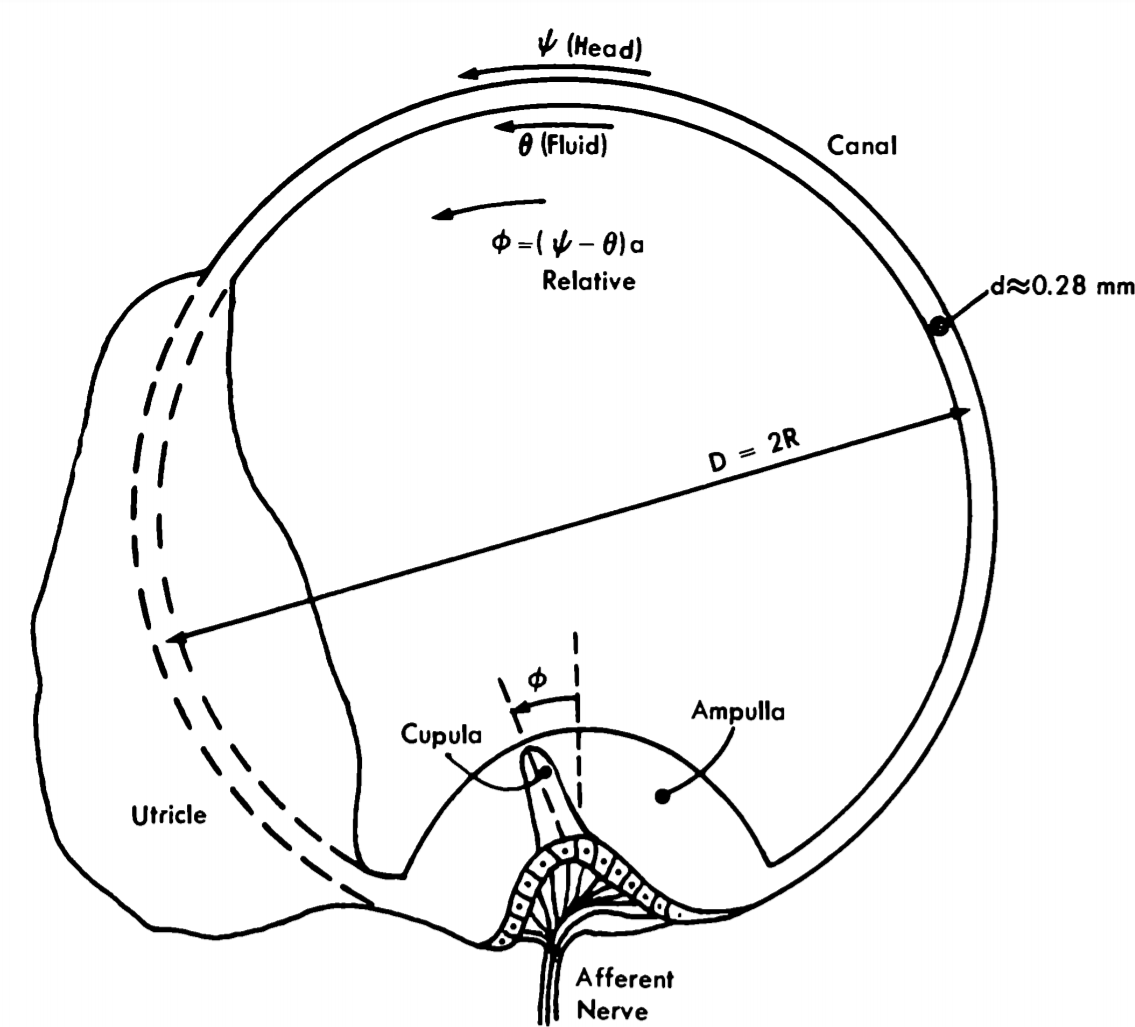
\includegraphics[scale=0.5]{The semicircular canal.png}
        \caption{The semicircular canal (diagrammatic)., \textbf{source:} from Jones and Milsum.}
    \end{figure}   
\begin{center}
 \begin{figure}[h]
        \centering
        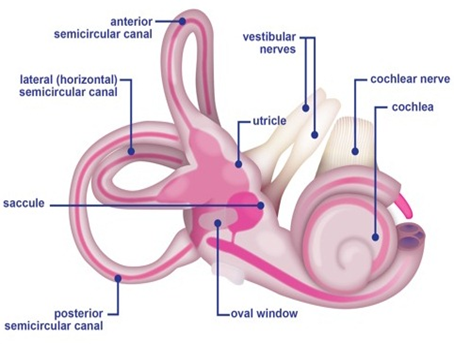
\includegraphics[scale=0.5]{inner-ear.png}
        \caption{3 perpendicular semicircular fluid canals in the inner ear, \textbf{source:} eyeandear.org.au}
    \end{figure}   
\end{center}
\newpage
\question{Real Analysis}{Let's see how the system is actually modeled!}
\part{1} There are 3 such canals (\textbf{corresponding to 3 spatial directions}) perpendicular to each other.
\\ \part{2} The fluid in them rotates slightly relative to the skull when the skull rotates in space and deflects the cupula.
\\ \part{3} The given analysis is based on angular motion in single plane.
\\ \part{4} LTI approximation as a second-order system:-
     \begin{itemize}
         \item \textbf{Fluid inertia:} The small bore of the canal ensures laminar flow
         \item \textbf{Viscous friction:} Viscous flow resistance is linearly dependent on velocity
         \item \textbf{Spring:} The cupula acts as a weak spring tending to restore itself
     \end{itemize}
\\ \part{5} Inertial frame equations:-
\begin{equation}
    b(\dot \Psi - \dot \theta) + k(\Psi - \theta) = J\ddot \theta 
\end{equation}
\begin{flushleft}
    \\where 
    \smallskip
    \\$\Psi=$ Absolute spatial position of skull
    \\ $\theta=$ Absolute spatial coordinate of the canal fluid
    \\J= moment of inertia of the fluid in the thin tube ($=mR^{2}$)
    \\b= torque per unit relative angular velocity 
    \\k= torque per unit relative angular displacement
    \end{flushleft}
\\ \part{6} But we are considered with the relative angular displacement $(\Psi - \theta)$ which produces the signal 9neural output).
\\ Hence, we get equation (1) as follows:
\begin{center}
    \[ J\ddot \phi (t) + b\dot \phi (t) + k\phi = (aJ)\ddot\Psi (t) \]
\end{center}
\\ \part{7} Let us write the transfer function as follows:-
\begin{center}
     \[{ \frac{\phi(s)}{\ddot \Psi(s)} = \frac{aJ}{Js^{2} + bs +k} } \]
    \[\Rightarrow\boxed{ \frac{\phi(s)}{\ddot \Psi(s)} = \frac{ k_{c} }{\frac{J}{k} s^{2} + \frac{b}{k} s + 1} } \]
\end{center}
\\ where, \(k_{c}= \frac{aJ}{k} \) is the steady-state gain.
\\ \part{8} For this system, natural frequency($ \omega_{n} $) is not very meaningful because of the \textbf{\textit{highly overdamped}} response characteristics. Consider:-
\begin{center}
    \[\boxed{ \frac{\phi(s)}{\ddot \Psi(s)} = \frac{ k_{c} }{(T_{1}s +1)(T_{2}s +1)} } \]
\end{center}
\\ Where, $T_{1}$ and $T_{2}$ can be considered as two first-order lags.
\begin{equation}
    T_{1} \cdot T_{2}= \frac{J}{k}
\end{equation}
\begin{equation}
    T_{1} + T_{2}= \frac{b}{k}
\end{equation}
\\ \part{9} In this particular case, $T_{1} \gg T_{2}$ .
\\The values for a man are as follows, which confirms the validity of our assumed approximations.
\[\boxed{T_{1}= 10 sec. , T_{2} = 1/200 sec. } \]
\question{References}
\smallskip
\\ \textbf{\textit{Reference 1:}} NISE, N. S. (2010), Control systems engineering, Wiley. (6$^{th}$ edition)
This is the course textbook.
\\ \textbf{\textit{Reference 2:}} MILSUM, J. S. (1966), Biological Control System Analysis, McGraw-Hill.
In this book, many other control systems like the pupil-control system and challenges for biological systems are also mentioned.
\end{document}